\documentclass[a4paper,14pt]{extarticle}
\usepackage{../../tex-shared/report-layout}

\begin{document}
\begin{titlepage}
    
    \thispagestyle{empty}
    
    \begin{center}
        
        Министерство науки и Высшего образования Российской Федерации \\
        Севастопольский государственный университет \\
        Кафедра ИС
        
        \vfill

        Отчет \\
        по лабораторной работе №\mylabnumber \\
        \enquote{\mylabtitle} \\
        по дисциплине \\
        \enquote{\MakeTextUppercase{\mysubject}}

    \end{center}

    \vspace{1cm}

    \noindent\hspace{7.5cm} Выполнил студент группы ИС/б-17-2-о \\
    \null\hspace{7.5cm} Горбенко К. Н. \\
    \null\hspace{7.5cm} Проверил \\
    \null\hspace{7.5cm} \mylecturer

    \vfill

    \begin{center}
        Севастополь \\
        \the\year{}
    \end{center}

\end{titlepage}

\section{Цель работы}
\begin{itemize}
    \item Приобрести базовые навыки работы в Deductor Studio;
    \item Изучить основы методов анализа экспериментальных данных и освоить
          технику их практического применения в Deductor Studio.
\end{itemize}

\section{Постановка задачи}
\begin{enumerate}
    \item Скачать и установить Deductor Studio Academic.
    \item Создать проект, заполнить его свойства, просмотреть файл проекта через
          любой текстовый редактор.
    \item Создать текстовый файл с данными, импортировать его в Deductor,
          настроить метки к столбцам, экспортировать файл, присоединить
          предыдущую ветвь к новому узлу импорта.
    \item Настроить следующие визуализаторы: \enquote{Таблица},
          \enquote{Статистика}.
    \item Ответить на контрольные вопросы.
    \item Подобрать данные и произвести поиск ассоциативных правил и
          прогнозирование временного ряда.
\end{enumerate}

\section{Изучение системы Deductor}
\subsection{Создание проекта}
Создадим проект в Deductor. Изменим его свойства и откроем в любом текстовом
редакторе. Сделаем видимой вкладку \enquote{Подключения}. Результат представлен
на рисунке \ref{fig:project-creation}.
\begin{figure}[H]
    \centering
    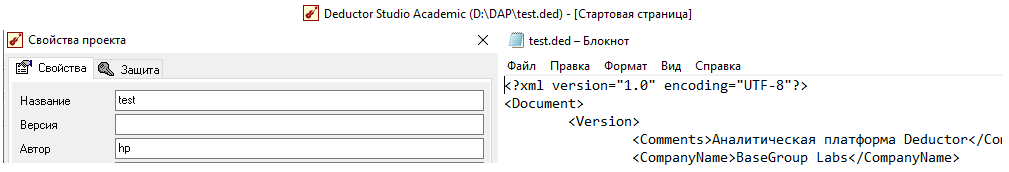
\includegraphics[width=\linewidth]{project-creation}
    \caption{Создание проекта в Deductor}
    \label{fig:project-creation}
\end{figure}

\subsection{Импорт и экспорт текстового файла}
Создадим текстовый файл и импортируем его в Deductor. После исправления в
программе экспортируем результат в текстовый файл и отобразим. Результат
представлен на рисунке \ref{fig:import-export}.
\begin{figure}[H]
    \centering
    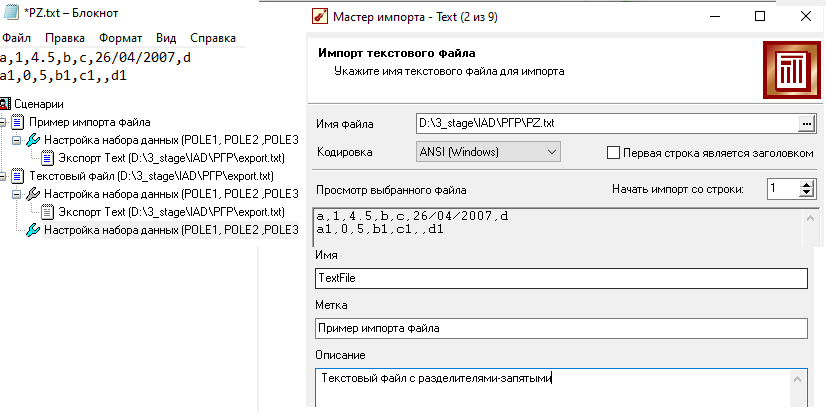
\includegraphics[width=.8\linewidth]{import-export}
    \caption{Импорт и экспорт в Deductor}
    \label{fig:import-export}
\end{figure}

\subsection{Настройка визуализаторов}
В проекте из предыдущего задания настроим визуализаторы. В визуализаторе таблицы
настроим, чтобы при отображении поля 3 добавлялась единица измерения. Результат
представлен на рисунке \ref{fig:visualizer}.
\begin{figure}[H]
    \centering
    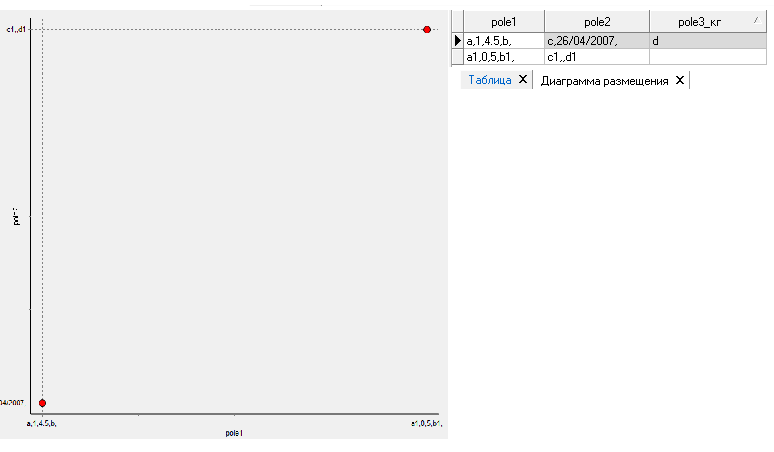
\includegraphics[width=.8\linewidth]{visualizer}
    \caption{Визуализаторы в Deductor}
    \label{fig:visualizer}
\end{figure}

\subsection{Ответы на контрольные вопросы}
\begin{enumerate}
    \item Дедуктор состоит из Warehouse, Studio, Viewer, Server, Client.
    \item Чтобы скрыть столбец из набора данных, нужно задать ему назначение
          \enquote{Неиспользуемое}.
    \item Категории пользователей: аналитик, пользователь, администратор,
          программист.
    \item Функции аналитика: создание в Deductor Studio сценариев –-
          последовательности шагов, которую необходимо провести для получения нужного
          результата, построение, оценка и интерпретация моделей, настройка панели
          отчетов для пользователей Deductor Viewer, настройка сценария на поточную
          обработку новых данных.
    \item В deductor studio ключевым понятием является проект. Это файл с
          расширением *.ded, по структуре соответствующий стандартному xml-файлу. Он
          хранит в себе последовательности обработки данных (сценарии),
          настроенные визуализаторы, переменные проекта и служебную информацию.
\end{enumerate}

\subsection{Выводы}
В ходе практической работы изучены основные возможности и компоненты программы
Deductor Studio. Изучены основные функции аналитиика, пользователя,
администратора, программиста в программе Deductor Studio.

\pagebreak
\section{Поиск ассоциативных правил}
\subsection{Подготовка данных}
В качестве исходных данных для анализа возьмем 30 чеков покупателей:
\begin{figure}[H]
    \centering
    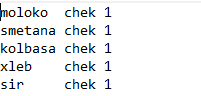
\includegraphics[width=.3\linewidth]{checks}
    \caption{Исходные данные}
    \label{fig:checks}
\end{figure}

\subsection{Составление таблицы}
Сформируем текущие данные в таблицу, состоящую из двух столбцов:
\enquote{Продукт} и \enquote{Номер чека} и укажем идентификатор и элемент
транзакции (рисунок \ref{fig:check-table}).
\begin{figure}[H]
    \centering
    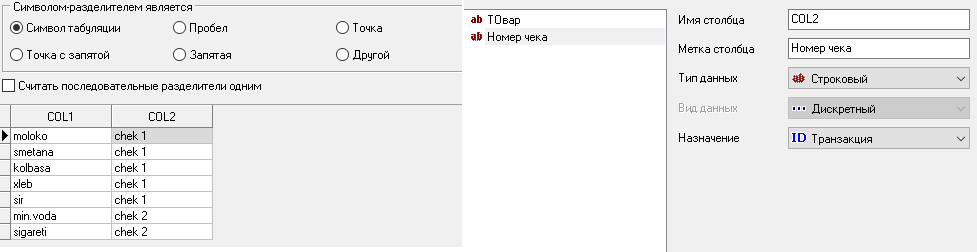
\includegraphics[width=\linewidth]{check-table}
    \caption{Определение столбца идентификатора транзакции и ее элемента}
    \label{fig:check-table}
\end{figure}

\subsection{Поиск ассоциативных правил}
Для поиска ассоциативных правил воспользуемся Мастером обработки, где выберем
тип обработки \enquote{Ассоциативные правила}.
\begin{figure}[H]
    \centering
    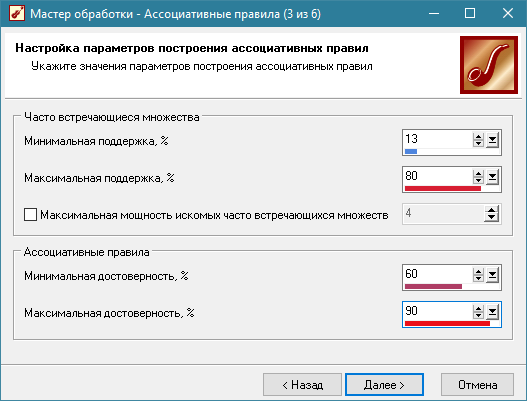
\includegraphics[width=.6\linewidth]{association-rules}
    \caption{Настройка параметров построения правил}
    \label{fig:association-rules}
\end{figure}

Последующие действия позволяет запустить процесс поиска ассоциативных правил.
Результат изображен на рисунке \ref{fig:association-result}.
\begin{figure}[H]
    \centering
    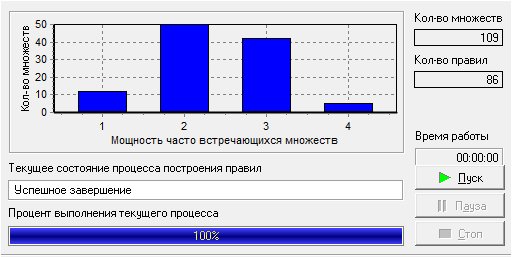
\includegraphics[width=.7\linewidth]{association-result}
    \caption{Результат поиска ассоциативных правил}
    \label{fig:association-result}
\end{figure}

\subsection{Определение популярных наборов}
Популярные наборы (рисунок \ref{fig:popular}):
\begin{figure}[H]
    \centering
    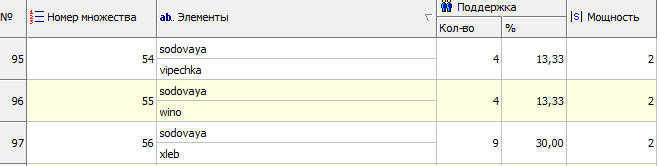
\includegraphics[width=\linewidth]{popular}
    \caption{Популярные наборы}
    \label{fig:popular}
\end{figure}
Исследуя визуализатор поиска ассоциативных правил \enquote{Популярные наборы}, можно
сделать вывод, что такие продукты, как колбаса, хлеб, минеральная вода являются
приоритетными к покупке в торговой точке.

\subsection{Визуализатор \enquote{Правила}}
Визуализатор \enquote{Правила} (рисунок \ref{fig:rules-visualizer}).
\begin{figure}[H]
    \centering
    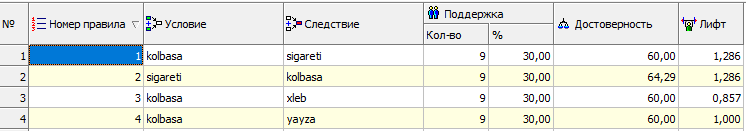
\includegraphics[width=\linewidth]{rules-visualizer}
    \caption{Визуализатор Правила}
    \label{fig:rules-visualizer}
\end{figure}
Из полученных результатов на рисунке 7 видно, что при покупке конфет, покупатель
с вероятностью 80\% купит и яйца и содовую, при покупке колбасы он купит сигареты
с вероятностью 60\%.

\subsection{Визуализатор \enquote{Дерево правил}} При построении дерева правил
по следствию на первом (верхнем) уровне находятся узлы со следствиями, а на
втором уровне – узлы с условиями.
\begin{figure}[H]
    \centering
    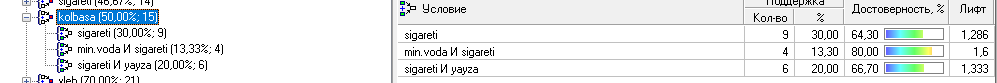
\includegraphics[width=\linewidth]{rules-tree}
    \caption{Построение дерева правил по следствию}
    \label{fig:rules-tree}
\end{figure}
Например, для того чтобы человек приобрел колбасу, он должен купить хотя бы один
предмет или несколько предметов из списка: сигареты, минеральную воду и
сигареты, сигареты и яйца.

Второй вариант дерева правил – дерево, построенное по условию. Здесь на первом
уровне располагаются узлы с условием (рисунок \ref{fig:rules-tree-by-condition}).
\begin{figure}[H]
    \centering
    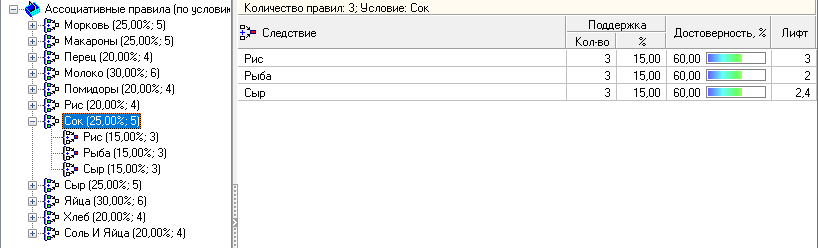
\includegraphics[width=\linewidth]{rules-tree-by-condition}
    \caption{Построение дерева правил по условию}
    \label{fig:rules-tree-by-condition}
\end{figure}
Узлы - верхний уровень дерева и условие. А ветви – следствия. Это означает, что
покупатель, купивший колбасу, так же купит сигареты, хлеб и яйца с
достоверностью 60\%.

\subsection{Анализ \enquote{Что-если}} Анализ “Что-если” позволяет определить,
что получим в качестве следствия, если выберем определенные условия. Например,
какие товары приобретаются совместно с выбранными товарами. Пусть необходимо
проанализировать, что, возможно, забыл покупатель приобрести, если он уже взял
сигареты и сметану.
\begin{figure}[H]
    \centering
    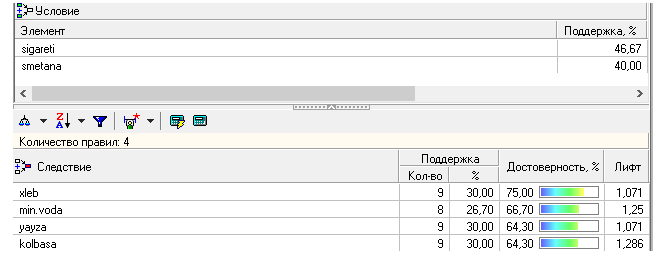
\includegraphics[width=\linewidth]{what-if}
    \caption{Результат анализа Что-Если}
    \label{fig:what-if}
\end{figure}
В данном случае появится минеральная вода, хлеб, яйца и колбаса. Именно эти
продукты покупатель возможно забыл приобрести с вероятностью 65-75\%.

\pagebreak
\section{Прогнозирование временного ряда}
\subsection{Импорт данных}
Для прогнозирования временного ряда были выбраны данные по продаже шампуня за
три года по месяцам:
\begin{lstlisting}
"Month","Sales"
"2018-01",266.0
"2018-02",145.9
"2018-03",183.1
"2018-04",119.3
"2018-05",180.3
"2018-06",168.5
"2018-07",231.8
"2018-08",224.5
"2018-09",192.8
"2018-10",122.9
...
\end{lstlisting}

Построим по исходным данным диаграмму:
\begin{figure}[H]
    \centering
    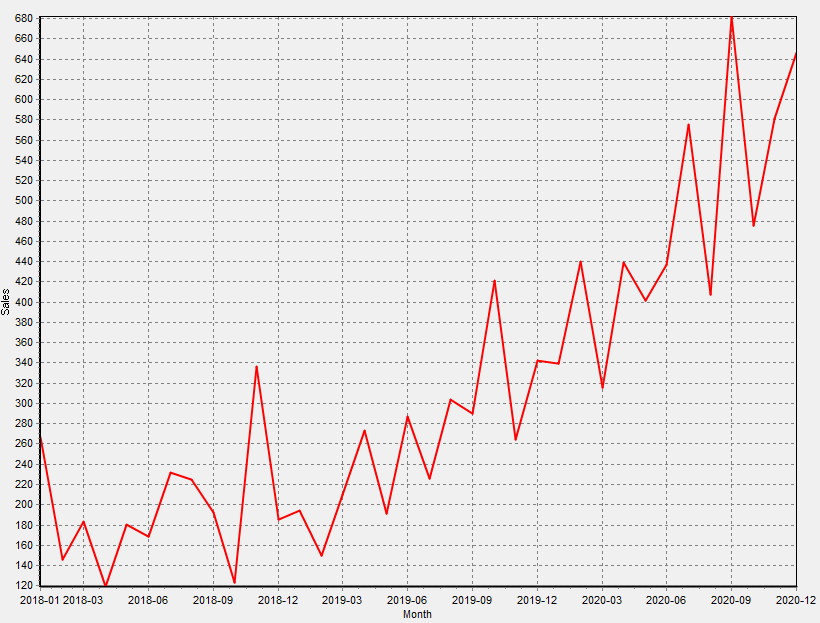
\includegraphics[width=.8\linewidth]{shampoo-diagram}
    \caption{Диаграмма, построенная по исходным данным}
    \label{fig:shampoo-diagram}
\end{figure}

\subsection{Обработка исходных данных}
По диаграмме видно, что в данных содержатся выбросы и шумы. Произведем
\enquote{Редактирование выбросов и экстремальных значений} и \enquote{Спектральную
обработку}. Результат представлен на рисунке \ref{fig:processed-shampoo-diagram}.
\begin{figure}[H]
    \centering
    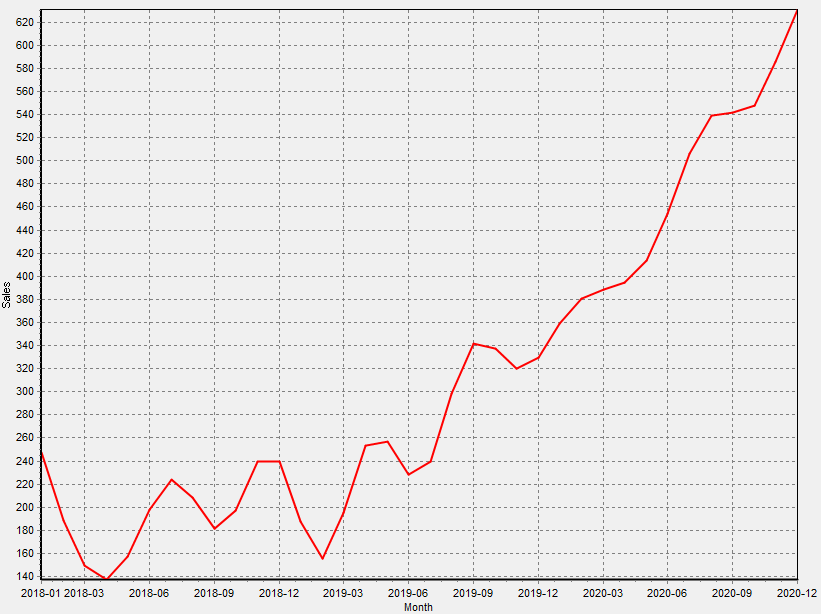
\includegraphics[width=.8\linewidth]{processed-shampoo-diagram}
    \caption{Диаграмма после обработки}
    \label{fig:processed-shampoo-diagram}
\end{figure}
Отберем данные используя метод \enquote{Скользящее окно} с глубиной погружения
12 месяцев. Результат представлен на рисунке \ref{fig:sliding-window}.
\begin{figure}[H]
    \centering
    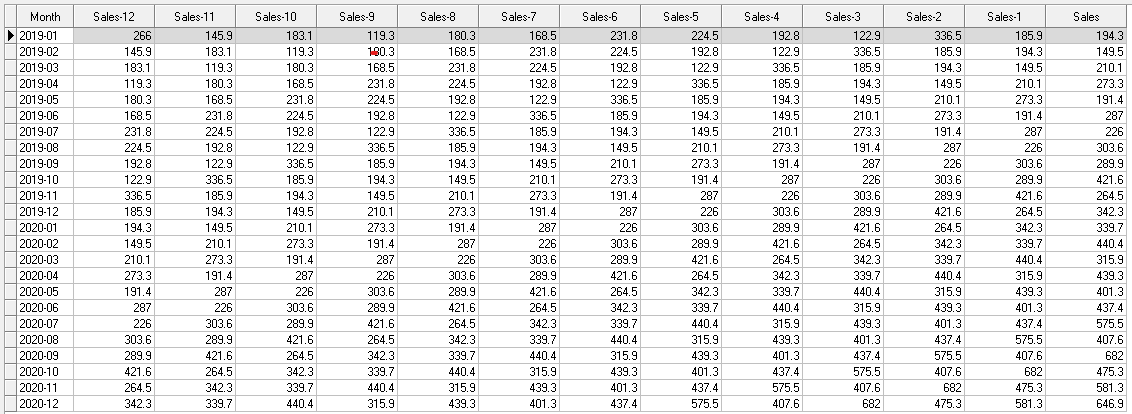
\includegraphics[width=\linewidth]{sliding-window}
    \caption{Результат работы метода \enquote{Скользящее окно}}
    \label{fig:sliding-window}
\end{figure}

\subsection{Обучение нейросети}
Воспользуемся мастером обработки, выберем в нем нейросеть. В качестве входных
полей используем первые 6 столбцов. Разобьем данные на тестовые и обучающие
Процесс изображен на рисунках \ref{fig:neuron-distribution} и \ref{fig:neuron-columns}.
\begin{figure}[H]
    \centering
    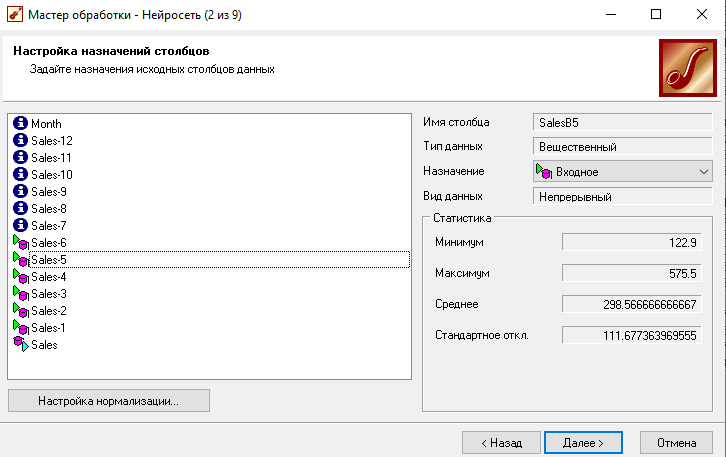
\includegraphics[width=.8\linewidth]{neuron-columns}
    \caption{Выбор столбцов входных данных для нейронной сети}
    \label{fig:neuron-columns}
\end{figure}
\begin{figure}[H]
    \centering
    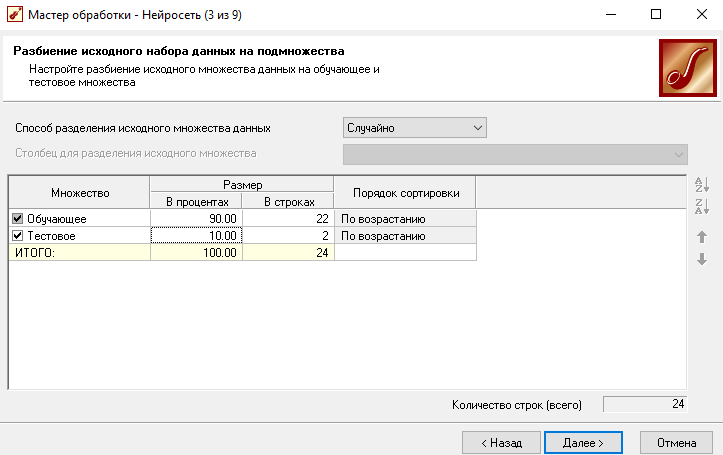
\includegraphics[width=.8\linewidth]{neuron-distribution}
    \caption{Распределение данных на обучающее и тестовое подмножества}
    \label{fig:neuron-distribution}
\end{figure}

Результат обучения нейросети представлен диаграммой рассеяния (рисунок
\ref{fig:diffusion-diagram}) и диаграммой, изображающей исходные данные вместе с
моделью, полученной с помощью нейросети (рисунок fig:neuron-vs-data):
\begin{figure}[H]
    \centering
    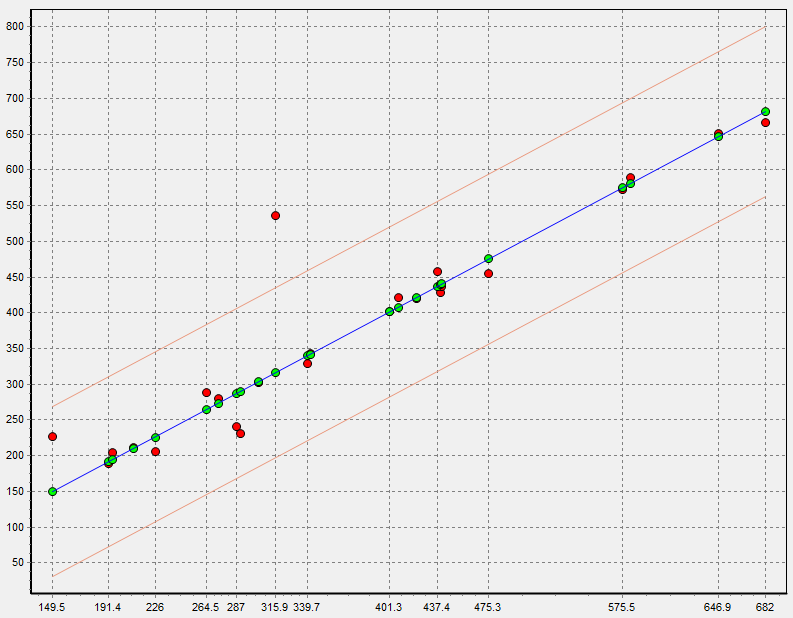
\includegraphics[width=.7\linewidth]{diffusion-diagram}
    \caption{Диаграмма рассеяния}
    \label{fig:diffusion-diagram}
\end{figure}
\begin{figure}[H]
    \centering
    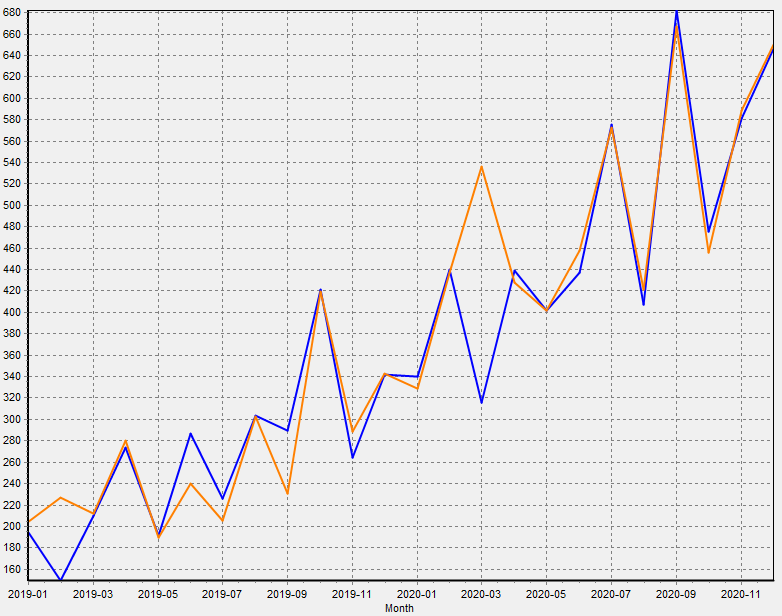
\includegraphics[width=.7\linewidth]{neuron-vs-data}
    \caption{Диаграмма по данным}
    \label{fig:neuron-vs-data}
\end{figure}
На диаграмме видно, что во втором месяц е 2018 г. и во втором месяце 2020 года
модель, построенная нейросетью не показывает реального падения в продажах.

\subsection{Прогнозирование продаж}
После того, как нейросеть была обучена, построим прогноз с помощью обработчика
\enquote{Прогнозирование}. Результат представлен на рисунке \ref{fig:prediction}.
\begin{figure}[H]
    \centering
    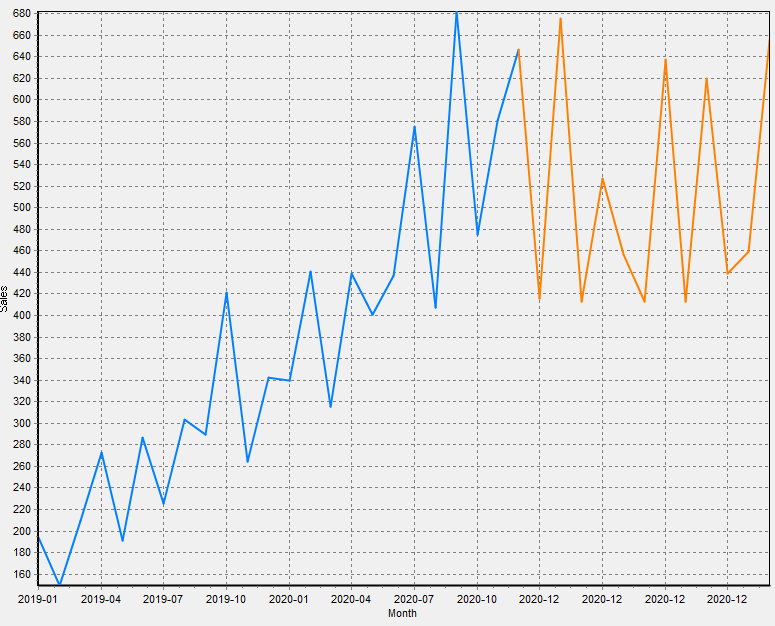
\includegraphics[width=.7\linewidth]{prediction}
    \caption{Прогноз продаж на 1 год}
    \label{fig:prediction}
\end{figure}
На диаграмме синим цветом (первые два года) изображены текущие продажи,
оранжевым цветом изображен прогноз продаж на год вперед.

\pagebreak
\section*{Выводы}
В ходе выполнения расчетно-графического задания был проведен поиск ассоциативных
правил для данных, представляющих собой чеки покупателей продуктового магазина.
Были выявлены популярные наборы: вода, картофель, колбаса, соль, яйца, лук,
молоко. В визуализаторах \enquote{Правила}, \enquote{Дерево правил} и
\enquote{Что-если} были определены условия и вероятности того, что приобретет
посетитель магазина, если он уже купил определенную товарную позицию в
магазине.

Также было проведено прогнозирование временного ряда количества продаж шампуня
за 3 года. При помощи \enquote{Редактирование выбросов и экстремальных значений}
и \enquote{Спектральная обработка} была проведена обработка данных от аномалий и
шумов, мешающих построению дальнейшей тенденции. Для прогнозирования временного
ряда при помощи нейросети было проведена обработка данных методом
\enquote{Скользящее окно} с глубиной погружения 12 месяцев. Проведено обучение
нейросети и построен прогноз продаж шампуня на год вперед.
\end{document}